\documentclass{article}

\usepackage{amssymb, amsmath, amsthm}
\usepackage[margin=1in]{geometry}
\usepackage{verbatim}
\usepackage{graphicx}
\usepackage{hyperref} % \url \href
\usepackage{docmute}
\usepackage[style=chem-acs ,backend=bibtex, sorting=none]{biblatex}
\usepackage{tikz}
\usepackage{blkarray}
\usepackage[title]{appendix}

\newtheorem{definition}{Definition}
\newtheorem{theorem}{Theorem}
\DeclareMathOperator{\spn}{Span}

\addbibresource{autoTB.bib}

\usetikzlibrary{shapes.geometric, arrows}
\tikzstyle{startstop} = [rectangle, rounded corners, minimum width=2cm,text centered, draw=black]
\tikzstyle{process} = [rectangle, minimum width=2cm, text centered, draw=black]
\tikzstyle{decision} = [diamond, minimum width=2cm, text centered, draw=black]
\tikzstyle{arrow} = [thick,->,>=stealth]

\begin{document}

    
\title{\emph{AutomaticTB}: Automatic Construction of Symmetry Adopted, Nearest Neighbor Tight-binding Model for Machine Learning}
\author{Wenhao Zhang}
\date{\today}
\maketitle

% this technique is given in https://tex.stackexchange.com/questions/87414/per-chapter-bibliographies-in-biblatex
\begin{refsection}
\documentclass{article}
\usepackage{amssymb, amsmath, amsthm}
\usepackage[margin=1in]{geometry}
\usepackage{verbatim}
\usepackage{graphicx}
\usepackage{hyperref} % \url \href
\usepackage{docmute}

\newtheorem{definition}{Definition}
\newtheorem{theorem}{Theorem}
\DeclareMathOperator{\spn}{Span}

\usepackage[style=chem-acs ,backend=bibtex, sorting=none]{biblatex}
\addbibresource{autoTB.bib}

\begin{document}

\section{INTRODUCTION}

It is inefficient to learn rules using try and error, while the rules can be 
simply stated. 
Similarly, if we want to achieve the best results using machine learning, which 
basically learn from statistic distribution of data, 
it is important that we include as much concrete rules as possible,
which should greatly improve the accuracy of ML prediction while simplify the 
problems for ML so that fewer data are necessary.

To let machines predict the energy levels of the electronic states of moleculars, for example,
one way is to input the molecular structure to ML and ask it to output the energies. 
However, this naive approach suffer from the problems that 1) this `ab-initio' approach
is too complicated to be formulated as a simple function that we can understand 
and 2) if we ourselves cannot understand it, it is more difficult for us to inspect the 
machine learning output: Is machine really learning anything important, or it just 
found some other patterns that fits the data but does not agree with our physical 
or chemical understanding?

Using results from group theory, it is possible to simplify the Hamiltonians of 
a molecular systems. Such approach utilize symmetry and provide
rules that quantum mechanical interactions have to obey. 
In the simplest case, a $s$ type wavefunction can not interact with a $p$ type wavefunction on the 
same atom, because their intergrals are strictly zero. 
Furthermore, group theory analysis force the degeneracy of the energy levels.
These informations reduce the size of the problem considerably. As a consequence, to 
find the energy of the states, we now only need to consider the remaining interactions 
that are allowed between MOs, and the problem is then largely 
an electro-static one, which should be simple enough for machine learning to solve.
We try to formulate the ideas in the following sections


\end{document}

\documentclass{article}
\usepackage{amssymb, amsmath, amsthm}
\usepackage[margin=1in]{geometry}
\usepackage{verbatim}
\usepackage{graphicx}
\usepackage{hyperref} % \url \href
\usepackage{docmute}
\usepackage{blkarray}

\newtheorem{definition}{Definition}
\newtheorem{theorem}{Theorem}
\DeclareMathOperator{\spn}{Span}

\usepackage[style=chem-acs ,backend=bibtex, sorting=none]{biblatex}
\addbibresource{autoTB.bib}


\begin{document}

\section{RELATED WORKS}

\end{document}
\newpage
\documentclass{article}
\usepackage{amssymb, amsmath, amsthm}
\usepackage[margin=1in]{geometry}
\usepackage{verbatim}
\usepackage{graphicx}
\usepackage{hyperref} % \url \href
\usepackage{docmute}
\usepackage{blkarray}

\newtheorem{definition}{Definition}
\newtheorem{theorem}{Theorem}
\DeclareMathOperator{\spn}{Span}

\usepackage[style=chem-acs ,backend=bibtex, sorting=none]{biblatex}
\addbibresource{autoTB.bib}

\usepackage{tikz}

\usetikzlibrary{shapes.geometric, arrows}
\tikzstyle{startstop} = [rectangle, rounded corners, minimum width=2cm,text centered, draw=black]
\tikzstyle{process} = [rectangle, minimum width=2cm, text centered, draw=black]
\tikzstyle{decision} = [diamond, minimum width=2cm, text centered, draw=black]
\tikzstyle{arrow} = [thick,->,>=stealth]

\begin{document}

\section{METHODS}

In this section, we first describe the tight-binding method, which yield the physical 
properties of the materials in concern. We next show, on the other hand, that using results 
from group theory and symmetry, the free parameters in a tight-binding model can be 
greatly reduced. The higher crystal symmetry, the smaller number of free parameters are 
necessary to describe the electronic structure. This is the key result in this work.

\subsection{AO and Tight-binding Method}
Tight-binding methods is a well known technique to solve the band structure of 
crystalline material with a model Hamiltonian\cite{ziman_principles_1999}. 
It is fast to run and is able to reproduce the DFT calculated band structure accurately 
provided a suitable set of parameters. In this section, we provide a short review of the 
basic methods.

In the tight binding approximation, we write the Hamiltonian in some \emph{local}
basis orbitals:
\begin{equation}
    H_{\mu\nu}(R) = \langle \chi_{R',\mu} | H | \chi_{R'+R,\nu} \rangle = \langle \phi_{0,\mu} | H | \phi_{R,\nu} \rangle
\end{equation}
we use $|\chi_{R,\mu}\rangle$ to denote an electronic states on atom $\mu$ in the cell indexed by lattice vector $R$. 
Due to periodicity, we can arbitrarily choose $R'$ to be zero and arrive at the simplified expression.
The Bloch-like basis functions are given by:
\begin{equation}
    |\psi_{\nu}^k\rangle = \sum_R e^{ik\cdot(R+t_{\nu})} |\phi_{R\nu} \rangle
\end{equation}
and the Hamiltonian matrix at reciprocal vector $\mathbf{k}$ is related to the 
Hamiltonian in real space by:
\begin{equation}
    \label{E:TB}
    H_{\mu\nu}^{\mathbf{k}} = \langle \psi_{\mu}^k | H |\psi_{\nu}^k\rangle = \sum_R e^{ik\cdot(R+t_{\nu}-t_{\mu})} H_{\mu\nu}(R)
\end{equation}
Diagonalizing the square matrix $H_{\mu\nu}^{\mathbf{k}}$ gives the eigen energies $\varepsilon_{\mathbf{k}}$s 
at $\mathbf{k}$ in the tight-binding approximation. 

An important point in the tight-binding approximation is that the interaction matrix elements in real
space should decay rapidly, so that the number of $R$ in the summation \eqref{E:TB} can be greatly 
reduced. In the extreme case, nearest neighbor interactions are considered only. 
The decay depend on the spatial extension of orbitals $|\phi_{R,\nu}\rangle$. 
The valid of this approximate therefore depend on the chemical nature of the bonding. In this work, we use 
atomic orbitals (AOs) as basis functions and assume nearest neighbor interaction only to reduce the 
number of parameters in the model. 

Given set of tight binding parameters $H_{\mu\nu}(R)$, crystal Hamiltonian can be diagonalized at any $k$ points. Therefore, 
band structure and density of states can be obtained straightforwardly. We use tetrahedron method to solve for 
the density of states on a regularly spaced $\mathbf{k}$-grid. 

\subsection{Molecular Orbitals}
In this and following sections, we take a detour to visit the notion of symmetry adopted molecular orbitals. 
For the following, we label atomic orbitals using $|\chi_{\mu}\rangle$ and molecular orbitals $|\psi_i\rangle$. The $i^{th}$ molecular 
orbital can be expressed as a linear combination of atomic orbitals (LCAO): 
\begin{equation}
    \label{E:MO_equation}
    \psi_i\rangle = c_{i\mu} |\chi_{\mu}\rangle + \cdots + c_{i\nu} |\chi_{\nu}\rangle
\end{equation}
As will be described later, we form the linear combinations from a set of symmetry equivalent orbitals, i.e., orbitals 
on equivalent atoms, in a local scope. Therefore, this linear combination is finite and relatively small. For simplicity,
we assume that the atomic orbitals on different atoms have ignorable overlap, then the normalization 
of molecular orbital given by equation \eqref{E:MO_equation} is simply given by the normalization of the 
coefficients $\sum_{\mu}c_{i\mu}^2 = 1$.

The interaction energies in atomic orbitals and molecular orbitals are also related by the coefficients $c_{i\mu}$ as:
\begin{equation}
    \label{E:HAO_HMO_transformation}
    H_{ij} = \sum_{\mu} \sum_{\nu} c_{i\mu} c_{j\nu} H_{\mu\nu}
\end{equation}
where $H_{ij}$ and $H_{\mu\nu}$ are the interaction in terms of molecular orbitals and atomic orbitals. 

\subsection{Symmetry Adapted Molecular Orbitals}
For the moment, we focus on isolated moleculars and discuss the properties of symmetry adopted molecular 
orbitals (symmetry adopted linear combinations, SALCs). Later we discuss the application of similar treatment 
in the case of crystal by focusing on local fragments. 

The symmetry operations of a molecular form a group and symmetry groups provide a way to label different functions 
by its irreducible representations. We provide some more details in the appendix. The conclusion here is 
that the eigenfunctions of the Hamiltonian are also labelled according to the irreducible representations. Functions 
that belong to different irreducible representations have different symmetry properties and their Hamiltonian 
matrix elements will be zero unless the two wavefunctions belong to the same type of irreducible representations:
\begin{equation}
    \langle \psi_i^{\Gamma_a} | H | \psi_j^{\Gamma_b} \rangle = \delta_{ab}
\end{equation}
Furthermore, the energy will be degeneracy for two wavefunctions in the same irreducible:
\begin{equation}
    \langle \psi_1^{\Gamma_a} | H | \psi_1^{\Gamma_a} \rangle = \langle \psi_2^{\Gamma_a} | H | \psi_2^{\Gamma_a} \rangle
\end{equation}
These properties of functions labelled by irreducible representation that we utilize to find the minimum 
interaction parameters. 

In moleculars, we can find a suitable set of basis functions so that single electron states can be 
expressed as a linear combination of them. The set of basis functions form a vector space within which we 
can find SALCs that corresponding to certain irreducible representations. Using groups' character table, 
we can define a projection operator that project out a subspace of a given irreducible representation $\Gamma_i$:
\begin{equation}
    P^{\Gamma_i} = \frac{l_i}{h} \sum_R \chi^{\Gamma_i}(R) P_R
\end{equation}
where $R$ is a group operation, $P_R$ operate on the given functions. 
$l_i$ is the dimension of the representation, $h$ is the order of the group and
$\chi^{\Gamma_i}(R)$ is the character. To start with, we find a spanning basis for the vector space, which 
are simply each individual atomic orbtials we include. Applying the projection operator to each of these 
orbitals yields all wavefunctions that has the same symmetry properties.

We use group $D_{3h}$ and planar molecular AH$_3$ as an example. The 
three dimensional vector space span by three $s$ functions on each H atoms
is given by:
\begin{equation}
    V = \spn(|\chi^s_{1}\rangle, |\chi^s_2\rangle, |\chi^s_3\rangle)
\end{equation}
Using the projection operator, we find two subspaces corresponding to representation $A_1'$ 
and $E'$ with basis:
\begin{align}
    | \psi_1^{A_1'} \rangle &= \frac{\sqrt{3}}{3} (|\chi^s_1\rangle + |\chi^s_2\rangle + |\chi^s_3\rangle) \\
    |\psi_2^{E'}\rangle   &= \frac{\sqrt{6}}{6}( 2|\chi^s_1\rangle - |\chi^s_2\rangle - |\chi^s_3\rangle) \\
    |\psi_3^{E'}\rangle   &= \frac{\sqrt{6}}{6}(- |\chi^s_1\rangle + 2|\chi^s_2\rangle - |\chi^s_3\rangle)
\end{align}
We note that the two basis for representation $E'$ is not orthogonal.
To explore the most from symmetries, we can further split the representation $E'$ into one
that is symmetric and antisymmetric under mirror reflection, by descending symmetry $D_{3h}\to C_s$ (subduction):
\begin{align}
    |\psi_2^{E'_{D_{3h}}\to A'_{C_s}} \rangle &= \frac{2}{\sqrt{6}} |\chi^s_2\rangle - \frac{1}{\sqrt{6}} |\chi^s_1\rangle - \frac{1}{\sqrt{6}} |\chi^s_3\rangle \\
    |\psi_3^{E'_{D_{3h}}\to A''_{C_s}}\rangle &= \frac{\sqrt{2}}{2} |\chi^s_1\rangle - \frac{\sqrt{2}}{2} |\chi^s_3\rangle
\end{align}
The symmetrized molecular orbitals formed by the three $s$ functions are shown on the right panel of Figure \ref{F:AH3_MO}

\begin{figure}[h!]
    \centering
    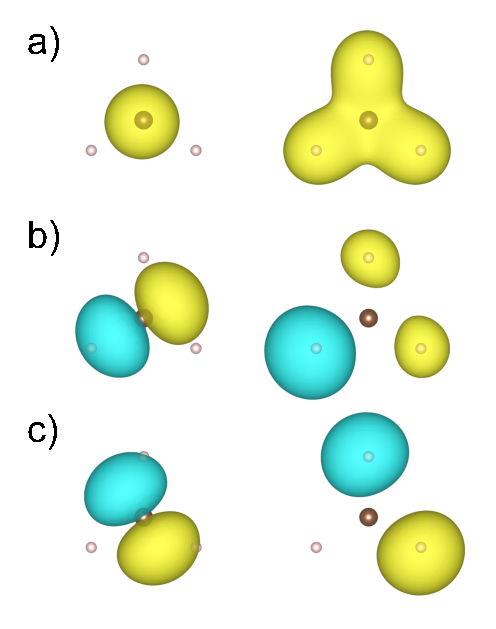
\includegraphics{../figures/AH3_MO.pdf}
    \caption{Interactions allowed between $s$ and $p$ orbitals on atom A and $s$ functions on H atoms,
        belonging to a) representation $A_1'$, b) $E' \to A'$ (symmetric with respect to mirror reflection)
        and c) $E'\to A''$ (antisymmetric with respect to mirror reflection) }
    \label{F:AH3_MO}
\end{figure}

We follow the same method for sites in crystals. Interested in local interactions, we focus on one atomic site at a time and its neighbors. 
The symmetry group is therefore given by the site symmetry group of that atomic site. 
There are in total 32 possible site symmetry (point) groups in crystal and all of their character tables can be obtained from Bilbao. 
We can separate all atomic orbitals in a such a local cluster into different symmetry equivalent orbitals and obtain the basis functions 
for each irreducible representations. 
The method to identify site syemmtry and characters for each site symmetry operation are provided in the supplementary. 
To perform symmetry descend to separate degenerate subspaces, we choose the suitable subgroups that are able to separate degenerate 
subspace into representations of different symmetry properties, following the subduction tables 
given in \cite{altmann_point-group_1994}. In principle, the input atomic orbital vectorspace can be splitted into 
one dimensional subspaces. Although there can be multiple functions correspond to the same symmetry type, they belong to distinct 
subspaces and will not mix under symmetry operation. On the other hand, symmetry operation will mix subspaces that are separated 
by symmetry descend, for example, a three fold rotation will mix $|\psi_2^{E'_{D_{3h}}\to A'_{C_s}} \rangle$ with 
$|\psi_3^{E'_{D_{3h}}\to A''_{C_s}}\rangle$, which is the reason for their energy degeneracy.

\subsection{Interactions Between Symmetrized MOs}
In this section, we seek to systematically describe the form of $H_{ij}$, the interaction between molecular orbitals. We 
label the symmetry adopted MOs using notation
\begin{equation}
    \psi^{\Gamma_i^{(\alpha)} \to \Gamma_m}_A
\end{equation}
where the superscript denote the symmetry properties. $\Gamma_i$ is the representation symbol of the site symmetry group. 
In general, there can be multiple subspace that belong to the same representation and we use $(\alpha)$ to index them. 
$\Gamma_m$ is the symbol of irreducible representation of the subgroup. \emph{This superscript uniquely identify all molecular 
orbitals found from the previous section}. 
Subscript denote the set of symmetry equivalent orbitals from which this molecular orbitals come from, 
for example, $p$ orbitals on equivalent atoms $j$, which help to specify
the nature of the molecular orbtials. We have the following symmetry restrains for $H_{ij}$:
\begin{equation}
    \langle \psi^{\Gamma_i^{(\alpha)} \to \Gamma_m} |  H | \psi^{\Gamma_j^{(\beta)} \to \Gamma_n} \rangle 
    = 0 \quad \text{unless } \Gamma_i = \Gamma_j\text{ and } \Gamma_m = \Gamma_n
\end{equation}
i.e., interactions are only allowed between molecular orbtials with the same symmetry and 
\begin{equation}
    \langle \psi^{\Gamma_i^{(\alpha)} \to \Gamma_m} |  H | \psi^{\Gamma_i^{(\beta)} \to \Gamma_m} \rangle 
    = \langle \psi^{\Gamma_i^{(\alpha)} \to \Gamma_n} |  H | \psi^{\Gamma_i^{(\beta)} \to \Gamma_n} \rangle 
    = \cdots
\end{equation}
so that the value of the interactions are the same for corresponding molecular orbitals with the same symmetry 
under two subspaces. This allow us to write the matrix $H_{ij}$ in a block form, with blocks between two 
representations of the site symmetry group $\Gamma_i^{(\alpha)}$ and $\Gamma_j^{(\beta)}$, which is a 
diagonal matrix with identical diagonal value ($a\cdot \mathbf{I}$) if $\Gamma_i = \Gamma_j$, and all zero otherwise. 

In the example of AH3 molecular, the interaction between MOs on A atoms and MOs from H can be write as follows:
\begin{equation}
    H_{ij} = \begin{blockarray}{cccc}
        % & |s^{A_1'}\rangle & |p_z^{A_2''}\rangle & |p_x^{E'}\rangle & |p_y^{E'}\rangle 
        & \psi^{A_1'}_{H,s} & \psi^{E'\to A'}_{H,s} & \psi^{E'\to A''}_{H,s} \\
        \begin{block}{c(ccc)}
        \psi^{A_1'}_{A,s}      & a & 0 & 0 \\
        \psi^{A_2''}_{A,p}     & 0 & 0 & 0 \\
        \psi^{E'\to A'}_{A,p}  & 0 & b & 0 \\
        \psi^{E'\to A''}_{A,p} & 0 & 0 & b \\
        \end{block}
        \end{blockarray}
\end{equation}
The interactions are shown in Figure \ref{F:AH3_MO}. Graphically, it is not easy to see that 
$\langle \psi^{E'\to A'}_{A,p} | H | \psi^{E'\to A'}_{H,s} \rangle = \langle \psi^{E'\to A''}_{A,p} | H | \psi^{E'\to A''}_{H,s} \rangle$,
we derive this relationship in the Appendix.


\subsection{Eliminating symmetry equivalent interactions}
We want to identify the minimum set of interations $H_{\mu\nu}$ which allow the generation of the entire tight-binding Hamiltonian, and we show 
here that the relationship between different $H_{\mu\nu}$s are encoded by $H_{ij}$. This procedure simplifies the size of 
the parameter finding problem as well as ensure the correct symmetry of the Hamiltonian. In the context of machine learning, recent advance in 
rotational invariant models automatically gives some relationship between different $H_{\mu\nu}$s, however, as illustrated by 
the following example, using representation theory, all symmetry relationship can be discovered in a systematic way. 

\begin{figure}[h!]
    \centering
    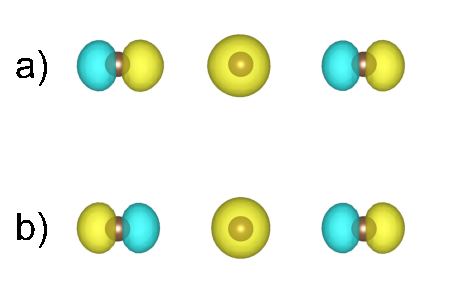
\includegraphics{../figures/S-Px.pdf}
    \caption{Interaction between $p_x^l \leftrightarrow s \leftrightarrow p_x^r$ on a linear molecular. 
                a) Interactions is not allowed by symmetry, and b) Interaction is allowed}
    \label{F:s_px_chain}
\end{figure}

We consider the simple case of $p_x^l \leftrightarrow s \leftrightarrow p_x^r$ interaction as shown in Figure \ref{F:s_px_chain}, 
where superscript $l$ and $r$ indicate left and right, in 
a site symmetry of $C_s$ (mirror). Suppose the interaction $s$--$p_x^r$ is $a$, it is apparent to us that the interaction $p_x^l$--$s$ is $-a$. However,
fact is not apparent for an rotational invariant machine learning model, because it is not possible to transform $p_x^l$
into $p_x^r$. 
On the second hand, due to symmetry, the two $p_x$ function can be combined into a symmetric and anti-symmetric part, and 
only the symmetric part interact with the $s$ function. So we have:
\begin{align}
    \label{E:px_s_AO_MO}
    \langle s | H | \psi_A'' \rangle = \frac{\sqrt{2}}{2} \left( \langle s | H | p_x^l \rangle + \langle s | H | p_x^r \rangle\right) = 0 \\
    \langle s | H | \psi_A' \rangle = \frac{\sqrt{2}}{2} \left( \langle s | H | p_x^l \rangle - \langle s | H | p_x^r \rangle\right) = b
\end{align}
which readily give the solution  $\langle s | H | p_x^l \rangle = \langle s | H | p_x^r \rangle = b/2$. 

When parameter $b$ is not known, we will have one equation only, in which case the value of $\langle s | H | p_x^l \rangle$ and 
$\langle s | H | p_x^r \rangle$ can not be solved. However, from the first equation, it is clear that only one of the two 
is free parameter. In more complicated case, free parameters can also be found in this way, since we can find a set of linear equations
\begin{gather}
    \sum_{\mu} \sum_{\nu} c_{1\mu} c_{2\nu} H_{\mu\nu} = H_{12} \\
    \sum_{\mu} \sum_{\nu} c_{1\mu} c_{3\nu} H_{\mu\nu} = H_{13} \\
    \cdots \\
    \sum_{\mu} \sum_{\nu} c_{i\mu} c_{j\nu} H_{\mu\nu} = H_{ij} 
\end{gather}
where many rows are zero on the right side, we can establish a homogeneous equation with number of rows $m$ less than number of 
unknown $n$. In such case, we will have in general $m-n$ free variables. To find these variable, we transform the 
coefficient matrix $C_{m\times n}$ into a row echelon form and each column without a leading variables would correspond to 
a free parameters. In this work, we use Gaussian elimination to bring the coefficient matrix to row echelon form.

\subsection{Generation of Tight-binding Hamiltonian}
Once suitable values are assigned to each of the free variables, values of all the unknowns can be found by appending to the homogeneous 
equation with rows, each has the free variables on the left and their corresponding on the right. This procedure produce a full rank 
coefficient and an linear equation system with unique solution. 

\begin{figure}[h!]
    \centering
    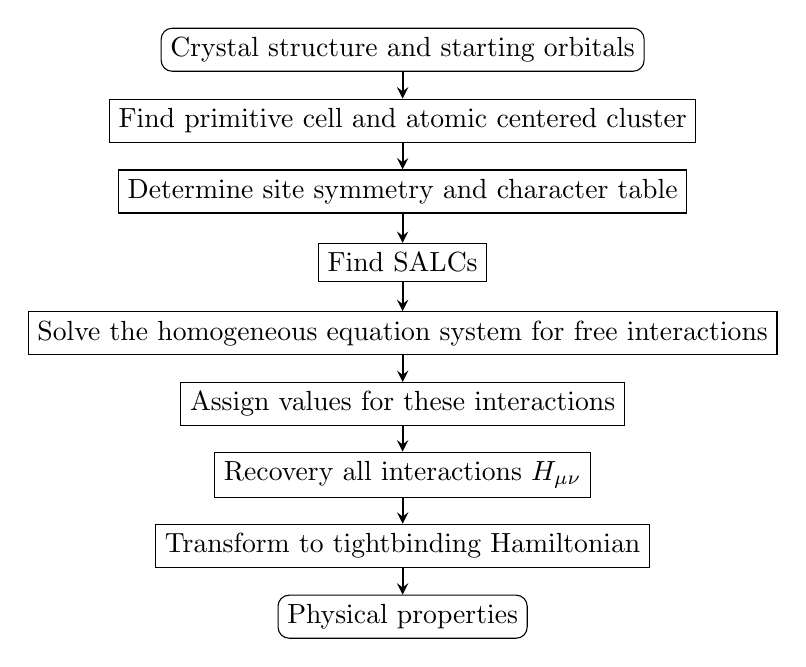
\begin{tikzpicture}[node distance=0.9cm]
        \node (start) [startstop] {Crystal structure and starting orbitals};
        \node (pro1) [process, below of=start] {Find primitive cell and atomic centered cluster};
        \draw [arrow] (start) -- (pro1);
        \node (pro2) [process, below of=pro1] {Determine site symmetry and character table};
        \draw [arrow] (pro1) -- (pro2);
        \node (pro3) [process, below of=pro2] {Find SALCs};
        \draw [arrow] (pro2) -- (pro3);
        \node (pro4) [process, below of=pro3] {Solve the homogeneous equation system for free interactions};
        \draw [arrow] (pro3) -- (pro4);
        \node (pro5) [process, below of=pro4] {Assign values for these interactions};
        \draw [arrow] (pro4) -- (pro5);
        \node (pro6) [process, below of=pro5] {Recovery all interactions $H_{\mu\nu}$};
        \draw [arrow] (pro5) -- (pro6);
        \node (pro7) [process, below of=pro6] {Transform to tightbinding Hamiltonian};
        \draw [arrow] (pro6) -- (pro7);
        \node (end) [startstop, below of=pro7] {Physical properties};
        \draw [arrow] (pro7) -- (end);
    \end{tikzpicture}
    \caption{Workflow of the generation of Tightbinding Hamiltonian}
    \label{F:workflow_Hamiltonian}
\end{figure}

To bring everything together, the workflow to generate the tight-binding Hamiltonian 
is organized as Figure \ref{F:workflow_Hamiltonian}. We start by finding atomic centered 
clusters and the vector space formed by the choosen starting basis. After finding 
site symmetry operations, we assign symmetry group and characters of each operations in the 
irreducible representations. The character table, together with subduction relationship, 
enable us to obtain the symmetry adopted molecular orbitals. The constrains 
given by symmetry allow us to reduce the number of free atomic interactions to the minimum 
number possible. Until this moment, there are no concrete values involved in the process.
Then, provided the values for each free atomic interactions, we are able to solve 
for all values of the interactions which we need for the formulation of tightbinding Hamiltonian.
After Hamiltonian in reciprocal space is obtained, electronic structure and derived properties 
can be extracted by solving the eigen values for the Hamiltonian. 

Our implementation is written in Python with numpy and are fully modulized. We provide solver 
for bandstructure with interface to Seekpath library for high symmetry k-path. Density of states
can be solved using tetrahedron summation method, provided with the code. We also offer 
interface to BoltzTrap2 for the solution of transport properties through linearized Boltzmann 
transport equations.

\end{document}

\documentclass{article}
\usepackage{amssymb, amsmath, amsthm}
\usepackage[margin=1in]{geometry}
\usepackage{verbatim}
\usepackage{graphicx}
\usepackage{hyperref} % \url \href
\usepackage{docmute}
\usepackage{blkarray}

\newtheorem{definition}{Definition}
\newtheorem{theorem}{Theorem}
\DeclareMathOperator{\spn}{Span}

\usepackage[style=chem-acs ,backend=bibtex, sorting=none]{biblatex}
\addbibresource{autoTB.bib}


\begin{document}

\section{Application}
\subsection{Tight-binding band structure in Pervoskite}

We describe the parameters in the cubic Halide Perovskite described in 
the work of Boyer et al.\cite{boyer-richard_symmetry-based_2016} as the 
our reference model. The parameters are as follows:
\begin{table}[h]
    \centering
    \caption{Tight binding parameters, Halide Perovskite Semiconductors}
    \label{T:TBP}
    \begin{tabular}{|c|c|c|}
        \hline
        Atom & Positions(crystal coord.) & Basis functions \\
        \hline
        B & $(0.0,0.0,0.0)$ & $|S_0\rangle$, $|X_0\rangle$, $|Y_0\rangle$, $|Z_0\rangle$ \\
        X & $(0.5,0.0,0.0)$ & $|S_1\rangle$, $|X_1\rangle$, $|Y_1\rangle$, $|Z_1\rangle$ \\
        X & $(0.0,0.5,0.0)$ & $|S_2\rangle$, $|X_2\rangle$, $|Y_2\rangle$, $|Z_2\rangle$ \\
        X & $(0.0,0.0,0.5)$ & $|S_3\rangle$, $|X_3\rangle$, $|Y_3\rangle$, $|Z_3\rangle$ \\
        \hline
    \end{tabular}
\end{table}
We have in total 16 atomic orbitals in the unit cell. In a $3\times 3\times 3$ supercell
which can include all the nearest neighbor interaction, We would have in total $N_s \times 16 \times 16$ parameters. 
Restricting the interaction to first order, only 304 interactions left. 
Now, we use the fact that orbitals belong to different symmetry cannot form bonding, 
so that matrix elements like $\langle S_0 | H | P_0 \rangle$ is zero, we can reduce the 
number of non-zero parameters. 
Finally, we use symmetry relationship to obtain relationship in bonding parameters. 
The interaction can be parameterized using only 9 parameters:
\begin{align*}
    E_{s0} &= \langle S_0 | H | S_0 \rangle \\
    E_{s1} &= \langle S_1 | H | S_1 \rangle \\
    E_{p0} &= \langle X_0 | H | X_0 \rangle \\
    E_{p1} &= \langle X_1 | H | X_1 \rangle 
\end{align*}
and 
\begin{align*}
    V_{ss} &= \langle S_0 | H | S_1 \rangle  \\
    V_{s0p1} &= \langle S_0 | H | X_1 \rangle \\
    V_{p0s1} &= \langle X_0 | H | S_1 \rangle \\
    V_{pp\sigma} &= \langle X_0 | H | X_1 \rangle \\
    V_{pp\pi} &= \langle Y_0 | H | Y_1 \rangle \\
\end{align*}

\end{document}
\newpage
\documentclass{article}
\usepackage{amssymb, amsmath, amsthm}
\usepackage[margin=1in]{geometry}
\usepackage{verbatim}
\usepackage{graphicx}
\usepackage{hyperref} % \url \href
\usepackage{docmute}
\usepackage{blkarray}

\newtheorem{definition}{Definition}
\newtheorem{theorem}{Theorem}
\DeclareMathOperator{\spn}{Span}

\usepackage[style=chem-acs ,backend=bibtex, sorting=none]{biblatex}
\addbibresource{autoTB.bib}


\begin{document}

\section{CONCLUSION}


\end{document}

\printbibliography[title={Reference}]

\end{refsection}


\begin{appendices}

\begin{refsection}
\documentclass{article}
\usepackage{amssymb, amsmath, amsthm}
\usepackage[margin=1in]{geometry}
\usepackage{verbatim}
\usepackage{graphicx}
\usepackage{hyperref} % \url \href
\usepackage{docmute}

\newtheorem{definition}{Definition}
\newtheorem{theorem}{Theorem}
\DeclareMathOperator{\spn}{Span}

\usepackage[style=chem-acs ,backend=bibtex, sorting=none]{biblatex}
\addbibresource{autoTB.bib}

\begin{document}

\section{Equivalent Interaction for AH3}
In this section, we show that, for the case of AH3, we have:
\begin{equation}
    \label{E:equivalent_AH3}
    \langle \psi^{E'\to A'}_{A,p} | H | \psi^{E'\to A'}_{H,s} \rangle = \langle \psi^{E'\to A''}_{A,p} | H | \psi^{E'\to A''}_{H,s} \rangle
\end{equation}
The following three interactions are related by a three fold rotation:
\begin{equation}
    \langle p_x | H | s_1 \rangle = \langle -\frac{1}{2}p_x + \frac{\sqrt{3}}{2}p_y | H | s_2 \rangle 
    = \langle -\frac{1}{2}p_x - \frac{\sqrt{3}}{2}p_y | H | s_3 \rangle
\end{equation}
where the three combinations of the $p$ orbitals on atom A points towards the three $s$ functions on the H atoms. We also have 
\begin{equation}
    \langle p_y | H | s_1 \rangle = \langle -\frac{\sqrt{3}}{2}p_x - \frac{1}{2}p_y | H | s_2 \rangle 
    = \langle \frac{\sqrt{3}}{2}p_x - \frac{1}{2}p_y | H | s_3 \rangle = 0
\end{equation}
where in this case, the $p$ orbitals points 90 degree to the $s$ functions and the interactions cancels.
Solving the above two equations, we have the following relationship:
\begin{gather}
    \label{E:AH3_relationship}
    \langle p_y | H | s_1 \rangle = 0 \\
    \langle p_x | H | s_1 \rangle = -2 \langle p_x | H | s_2 \rangle = -2 \langle p_x | H | s_3 \rangle = 
    \frac{\sqrt{3}}{3} \langle p_y | H | s_2 \rangle = - \frac{\sqrt{3}}{3} \langle p_y | H | s_3 \rangle
\end{gather}
Using there relationships, we can find:
\begin{align}
   \frac{\sqrt{6}}{6} \langle p_x | H | 2 s_1 -  s_2 -  s_3 \rangle &= \frac{\sqrt{6}}{2} \langle p_x | H | s_1 \rangle \\
   \frac{\sqrt{2}}{2} \langle p_y | H | s_2 -  s_3 \rangle &= \frac{\sqrt{6}}{2} \langle p_x | H | s_1 \rangle 
\end{align}
showing that the two interaction given in equation \eqref{E:equivalent_AH3} indeed have the same value. 
We comment that the relationship given in equation \eqref{E:AH3_relationship} are the same as the relationship 
recoveried using the symmetry restrains and solving the homogeneous equations, as mentioned in the 
article. However, the method here is rather ad-hoc. For example, it is not clear why the values such as 
$\langle \frac{\sqrt{3}}{2}p_x - \frac{1}{2}p_y | H | s_3 \rangle$ is zero without carrying out intergral (although 
it is apparent by visual inspectations). The constrains solved from interactions between symmetrized molecular 
functions, however, are systematic. 

\end{document}
\documentclass{article}
\usepackage{amssymb, amsmath, amsthm}
\usepackage[margin=1in]{geometry}
\usepackage{verbatim}
\usepackage{graphicx}
\usepackage{hyperref} % \url \href
\usepackage{docmute}

\usepackage{tikz}
\usetikzlibrary{shapes.geometric, arrows}
\tikzstyle{startstop} = [rectangle, rounded corners, minimum width=2cm,text centered, draw=black]
\tikzstyle{process} = [rectangle, minimum width=2cm, text centered, draw=black]
\tikzstyle{decision} = [diamond, minimum width=2cm, text centered, draw=black]
\tikzstyle{arrow} = [thick,->,>=stealth]

\newtheorem{definition}{Definition}
\newtheorem{theorem}{Theorem}
\DeclareMathOperator{\spn}{Span}

\newtheorem{definition}{Definition}
\newtheorem{theorem}{Theorem}
\DeclareMathOperator{\spn}{Span}

\usepackage[style=chem-acs ,backend=bibtex, sorting=none]{biblatex}
\addbibresource{autoTB.bib}

\begin{document}

\section{Character table for site symmetry groups}

To use symmetry information in the construction of a tight-binding model, we first need to 
find the concrete symmetry group and it's representations. 
In this section, our implementation to find the site symmetry group in crystal, as well as 
its subgroups and characters are described in details.

\subsection{Basic Definition}

For a point $\mathbf{x}$ in a crystal, the subgroup of the space group $G$ that leave $\mathbf{x}$
fixed is called the \emph{site symmetry groups}, which we denote $S_{\mathbf{x}}$. A space group
operation in crystal can be denoted using matrix--column pair $(\mathbf{W},\mathbf{w})$ in a chosen 
basis. Then it is straightforwardly to see that group elements in the site symmetry group only 
contain rotation part. 

Given a rotation matrix $\mathbf{W}$ belonging to a site symmetry group, it can be classified into different
types, each designated by their Hermann--Mauguin (HM) symbols, depending on its trace and determinant. 
The trace $\text{tr}\mathbf{W}$ give information of the rotation angle and determinant indicates whether 
the operation is first or second kind. 
Since trace is invariant under permutation of matrices, it does not depend on any change of basis. 
They are listed in Table \ref{T:operation_properties}. 

\begin{table}[h!]
    \centering
    \caption{Site symmetry types}
    \begin{tabular}{|c|cccccccccc|}
        \hline
        $\det$      & +1 & +1 & +1 & +1 & +1 & -1 & -1 & -1 & -1 & -1 \\ 
        $\text{tr}$ &  3 &  2 &  1 &  0 & -1 & -3 & -2 & -1 &  0 &  1 \\  
        \hline
        type        &  1 &  6 &  4 &  3 &  2 & -1 & -6 & -4 & -3 & -2 = m \\ 
        \hline
    \end{tabular}
    \label{T:operation_properties}
\end{table}

There are in total 32 crystallographic point group types so that the number of distinct site symmetry group types are
also limited to 32. They can be easily identified by counting the types of operation in the group. 
Reference table can be found in Togo and Tanaka\cite{togo_spglib_2018}.

For point groups, its group operation can be uniquely denoted using \emph{Seitz symbols}. The Seitz symbol consists of 
three parts: 1) HM symbol of the operation, 2) its characteristic direction denoted by $[uvw]$ and 3) the sense of rotation $+$ or $-$. 
The sense of rotation indicate whether the rotation is clockwise or anti-clockwise and is used for $4$, $-4$, $3$, $-3$, $6$, $-6$ only.
The characteristic direction (lattice direction) is usually given with respect to different lattice systems. We use hexagonal lattice 
for both hexagonal and rhombohedral lattice. The basis for each lattice can be found in Section 2.2 of \emph{ITA}. 

the number of possible site symmetry is greatly reduced compared to 
that in the moleculars. Possible rotations can be characterized by the trace 
and determinant of the rotation matrix, where the $\det\mathbf{W}$ indicate the 
existance of inversion in the operation and $\text{tr}\mathbf{W}$ gives the angle of rotation. 
Since trace is invariant under permutation, angle of rotation does not depend on the 
basis vector of the symmetry matrix. The characterization is listed by table \ref{T:operation_properties}.

\subsection{Finding the Seitz symbol from Operation Matrix}


The total number of crystallographic point groups in three dimension is 32, and their character tables are 
tabulated either in The point group table of the bilbao crystallographic server \href{https://www.cryst.ehu.es/rep/point.html}{bilbao}. 
In crystallographic server, all the matrix element of the operations are also given explicitly, in the respective basis vector 
and denoted in Seitz symbol. Their characters can also be found from the same webpage.
Seitz symbols are tabulated as well (Seitz symbols for crystallographic symmetry operations)
with the standard basis vectors given in the international table for each crystal system. 
In our implementation, the character table of the 32 point symmetry groups are taken from bilbao server and 
stored. For hexagonal lattice, we use the hexagonal setting.

However, one complication arise when the site symmetry operation does not correspond to the standard basis. For example, 
in a cubic crystal belong to space group $Pm\bar{3}m$ (221), the point $(x,x,x)$ on the body diagonal has site symmetry $3m$
whose rotation matrix is tabulated in hexagonal basis. Therefore, we cannot directly compare the rotation matrix of the 
site symmetry operation with the ones tabulated in the Bilbao server. Instead, we use the following method to generate 
the seitz symbol from a list of rotation matrices, and then use the seitz symbol to assign characters to each symmetry 
operations. The input rotation matrices can correspond to any orientation.

A seitz symbol consist of three parts: type of the symmetry operation, sense of the rotation 
(for rotation $4$, $-4$, $3$, $-3$, $6$, $-6$ only) and the characteristic direction. 
Symmetry type can be found according to table \ref{T:operation_properties}. To find the 
symmetry direction in the standard basis, we first find the symmetry direction in the cartesian coordinate. 

For symmetry $1$ or $\bar{1}$, a point $(0.0, 0.0, 0.0)$ will be assigned. If the symmetry operation is a rotoinversion,
we multiplicity it by $-\mathbf{1}$ to obtain the rotation parts $\mathbf{W}$. 
The symmetry direction is given by finding the eigenvector with eigenvalue $1$. 
\begin{equation}
    \label{E:rotation_axes}
    \mathbf{W}\mathbf{v} = \mathbf{v}
\end{equation}

After computing the directions of all the symmetry operation, we separate them into sets that are related by symmetry operations:
\begin{equation}
    \{\mathbf{v}' \mid \mathbf{W}\mathbf{v}, \mathbf{W} \in \mathbf{R}\}
\end{equation}
All symmetry direction belonging to the same set contain the same symmetry elements, and they correspond to the symmetry directions 
used in Hermann--Mauguin symbol. For example, the result of the classification is listed in table \ref{T:6mmm} for group $6/mmm$
\begin{table}[h]
    \centering
    \caption{Symmetry operation and directions in cartesian coordinate in $6/mmm$}
    \begin{tabular}{|c|l|l|}
        \hline
        Operation & Directions & Symmetry Direction\\
        \hline
        -1,1 & (  0.0  0.0  0.0) & $\mathbf{0}$\\
        6,-3,-6,m,2,3 & (  0.0  0.0  1.0) & $[001]$\\
        m,2 & (-0.5,-0.866,0.0), (1.0,0.0,0.0), (-0.5,0.866,0.0) & $[100],[010],[\bar{1}\bar{1}0]$\\
        m,2 & (0.866,-0.5,0.0), (0.0,1.0,0.0), (-0.866,-0.5,0.0) & $[120],[\bar{2}\bar{1}0],[1\bar{1}0]$\\
        \hline
    \end{tabular}
    \label{T:6mmm}
\end{table}

Then, it is possible to choose the basis for the site symmetry group. The choice of 
the axes are listed in table \ref{T:choice_of_axes}. 
After choosing $\mathbf{a}$ and $\mathbf{b}$, $\mathbf{c}$ is chosen so that the three axes
form a right-handed system: $(\mathbf{a}\times \mathbf{b}) \cdot \mathbf{c} > 0$. 
The direction in cartesian coordinates corresponding to the symmetry direction in the seitz symbol can also be computed and can be 
compared to the symmetry direction found using equation \eqref{E:rotation_axes}. Finally, the 
sense of the rotation can be computed using the method provided by 
\emph{Efficient conversion from rotating matrix to rotation axis and angle by extending Rodrigues’ formula},
by calculating the $\sin\theta$. 

\begin{table}[h]
    \centering
    \caption{Choice of $\mathbf{a}$, $\mathbf{b}$ and $\mathbf{c}$}
    \begin{tabular}{|c|c|}
        \hline
        Groups & Choice\\
        \hline
        \begin{tabular}{c}$2$, $m$, $2/m$, $4$, $-4$, $4/m$\\$3$, $-3$, $6$, $-6$, $6/m$\end{tabular}
            & $z = [001]$ \\ \hline
        $222$, $mm2$, $mmm$ & $x=[100],y=[010],z=[001]$ \\\hline
        $32$, $3m$, $-3m$, $622$, $6mm$, $-6m2$, $6/mmm$ & $\{x, y\} \in \{[100], [010],[\bar{1}\bar{1}0]\}$ \\\hline
        $23$, $m-3$, $432$, $-43m$, $m-3m$ & $\{x,y,z\} = \{[100],[010],[001]\}$ \\
        \hline
    \end{tabular}
    \label{T:choice_of_axes}
\end{table}


\begin{figure}[h]
    \centering
    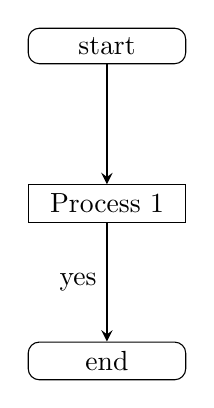
\begin{tikzpicture}[node distance=2cm]
        \node (start) [startstop] {start};
        \node (pro1) [process, below of=start] {Process 1};
        \draw [arrow] (start) -- (pro1);
        \node (end) [startstop, below of=pro1] {end};
        \draw [arrow] (pro1) -- node[anchor=east] {yes} (end);
    \end{tikzpicture}
    \caption{Workflow}
    \label{F:workflow}
\end{figure}

\subsection{Symmetry reduction}
In our application, we need to find the subgroup of the site symmetry group so that we can separate basis 
uniquely for a representation with more than one dimension. To do so, we need to know which symmetry is 
kept when we move from a group to its subgroup. Finding the subgroups is not a trivial task and we 
manually assign maps from the seitz symbol of the subgroup to the ones in the supergroup. In this way, subgroup
and the correspond characters are readily obtained onces the seitz symbol of the site-symmetry group is known.

\subsection{Subduction}
Subduction enable us to perform symmetry descend that split the irreducible representation into 
different subspaces with different symmetry. 

\end{document}

\documentclass{article}
\usepackage{amssymb, amsmath, amsthm}
\usepackage[margin=1in]{geometry}
\usepackage{verbatim}
\usepackage{graphicx}
\usepackage{hyperref} % \url \href
\usepackage{docmute}

\newtheorem{definition}{Definition}
\newtheorem{theorem}{Theorem}
\DeclareMathOperator{\spn}{Span}

\usepackage[style=chem-acs ,backend=bibtex, sorting=none]{biblatex}
\addbibresource{autoTB.bib}

\begin{document}

\section{Groups, representations and basis}
\subsection{Groups and representations}
The symmetry operation that map a molecular onto itself form a group $G$. From a group,
we define a representation of group $G$ as a mapping:
\begin{definition}
    A linear \emph{representation} of a group $G$ on a vector space $V$ is a homomorphism:
    \[\rho\colon G \to \text{GL}(V)\]
    where homomorphism is a mapping that satisfies $\rho(g_1g_2) = \rho(g_1)\rho(g_2)$.
\end{definition}
Representations are not unique: a change of basis leads to an equivalent representation 
and the direct sum of two representation is again a representation. However, representations
can be uniquely reduced to so called \emph{irreducible representations}.
We define the notion of \emph{invariant vector space}:
\begin{definition}
    For any vector $v$ in $V$, for any $g\in G$, if we have $\rho(g)v \in V$, then $V$
    is an invariant vector space.
\end{definition} 
For a representation with vector space $V$, $V$ is an invariant to the group $G$. 
If there exist a vector space $W\subset V$ which is also invariant to $G$, then we call $W$
an \emph{invariant subspace}. 
Furthermore, there exist another invariant subspace $U$ of $V$ so that $V$ is given by a direct sum:
\begin{equation}
    V = U \oplus W
\end{equation}
By splitting the vector space $V$ into invariant subspaces until it is not possible, we find the 
\emph{irreducible representation} by the reducible representation on $V$, and the matrix form 
of the reducible representation can be written as the block diagonal form
\begin{equation}
    \rho^{\Gamma}(g) = \left(  
        \begin{matrix}
            \rho^{\Gamma_1} (g) & 0 & \cdots\\
            0 & \rho^{\Gamma_2} (g) & \\
            \vdots &  & \ddots
        \end{matrix}
    \right)
\end{equation}
where $\Gamma$ denote the reducible representation and $\Gamma_i\ (i = 1, \dots)$ index 
the irreducible representations.

\subsection{Basis functions}
For each invariant subspaces corresponding to a representation $\Gamma_n$, we write its basis 
functions using the braket notation $|\Gamma_n,j\rangle$. For a irreducible representation with 
dimension $N$, we have $N$ such basis functions and any vectors in this invariant subspace 
can be written as a linear combination:
\begin{equation}
    |\phi^{\Gamma_n}\rangle = \sum_{i = 1}^N c_i |\Gamma_n,i\rangle
\end{equation} 
Due to the definition of invariant subspace, the matrix representation of $G$ in the invariant 
subspace will have the form:
\begin{equation}
    \rho^{\Gamma_n}(g)_{ij} = \langle \Gamma_n,i | P_g | \Gamma_n,j \rangle
\end{equation}
where $P_g$ is the symmetry operation. 
For reducible representations $\Gamma_{r}$, its vector subspace is a direct sum of all the subspace 
of irreducible representations it contains. Therefore, basis functions from irreducible 
subspaces together form the basis functions for the reducible representation.

The basis functions of the representation of the symmetry group is closely connected to quantum mechanics.
Since the Hamiltonian of the system is invariant to the symmetry operation, we have the commutation 
relationship:
\begin{equation}
    [P_g,H] = 0
\end{equation}
for any symmetry operation $g$. As a consequence, if $|\phi_{\varepsilon_i}\rangle$ an eigenfunction of $H$
with eigenvalue $\varepsilon_i$, $P_g|\phi_{\varepsilon_i}\rangle$ will also be an eigenfunction 
with degenerate eigenvalues. Since $|\phi_{\varepsilon_i}\rangle$ and $P_g|\phi_{\varepsilon_i}\rangle$
together will define some invariant space. Therefore, it is possible to classify the eigenfunctions of the 
Hamiltonian according to the subspaces which they occupy, and the set of degenerate eigenfunctions are 
related by symmetry operation. 

\end{document}

\documentclass{article}
\usepackage{amssymb, amsmath, amsthm}
\usepackage[margin=1in]{geometry}
\usepackage{verbatim}
\usepackage{graphicx}
\usepackage{hyperref} % \url \href
\usepackage{docmute}

\newtheorem{definition}{Definition}
\newtheorem{theorem}{Theorem}
\DeclareMathOperator{\spn}{Span}

\usepackage[style=chem-acs ,backend=bibtex, sorting=none]{biblatex}
\addbibresource{autoTB.bib}

\begin{document}

\section{Finding the representations and Symmetry adopted basis functions}
\subsection{Molecular orbitals}
Using character table and the orthogonality theorem for characters, we can find the basis functions 
of the Hamiltonians knowing only the symmetry property of the structure. 

We start by finding the vector space of all the participating atomic orbitals and their transformation 
properties under group operation, then we decompose the reducible representation to irreducible ones. 
We follow the example of Dresselhaus\cite{dresselhaus_group_2008} and consider the group $D_{3h}$ with 
the following character table \ref{T:ct}
\begin{table}[h!]
    \centering
    \caption{Character table of $D_{3h}$}
    \begin{tabular}{|c|c|c|c|c|c|c|}
        \hline
                & $E$ & $\sigma_h$ & 2$C_3$ & 2$S_3$ & 2$C_2'$ & 3$\sigma_v$ \\ \hline
         $A_1'$ &  1  &  1         &  1     &  1     &   1     &   1         \\
         $A_2'$ &  1  &  1         &  1     &  1     &  -1     &  -1         \\
         $A_1''$&  1  & -1         &  1     & -1     &   1     &  -1         \\
         $A_2''$&  1  & -1         &  1     & -1     &  -1     &   1         \\
         $E'$   &  2  &  2         &  -1    & -1     &   0     &   0         \\
         $E''$  &  2  & -2         &  -1    &  1     &   0     &   0         \\ \hline
    \end{tabular}
    \label{T:ct}
\end{table}

Suppose we have four atoms, one on the rotation axis and three other that transform to each other 
by three fold rotation, and $s$ and $p$ orbitals on each of the atoms. Indexing each atomic 
centered functions using atomic index $i$ and orbital index $l,m$ as $| i,l,m \rangle$ 
(or $| i,s \rangle, \dots, |i,p_x\rangle$ if convenient), we form 
a vector space with dimension $4\times4 = 16$:
\begin{equation}
    V = \spn(| 1,s \rangle, | 1,p_x \rangle ,\dots, | 4,p_y \rangle, | 4,p_z \rangle)
\end{equation}
We can find the matrix elements of the symmetry group in this space using the following equation:
\begin{equation}
    \rho(g)_{ij} = \langle i | P_g | j \rangle
\end{equation}
where $\rho(g)$ is the matrix in the vector space of atomic basis function and $P_g$ is the 
operators that transform the basis functions. 
After generating the matrix of each symmetry operation, we find the character of the representation
in this atomic orbital basis:
\begin{gather*}
    \chi^{AOs}(E) = 16,\ \chi^{AOs}(\sigma_h) = 8,\ \chi^{AOs}(C_3) = 1\\ 
    \chi^{AOs}(S_3) = -1,\ \chi^{AOs}(C_2') = 0,\ \chi^{AOs}(\sigma_v) = 4
\end{gather*}
The uniqe decomposition of the reducible representation into the irreducible ones are given by:
\begin{gather}
    a_i = \frac{1}{h} \sum_{k} N_k \chi^{\Gamma_i}(C_k)^* \chi(C_k)
\end{gather}
Decomposing the above represention in atomic orbital space, we obtain the following relationship:
\begin{equation}
    \Gamma^{AOs} = 
      3\Gamma^{A_1'} + \Gamma^{A_2'}  + 2\Gamma^{A_2''} + 4\Gamma^{E'} + \Gamma^{E''}
\end{equation}

\subsection{Projecting into Vector Space of Irreducible Representation}
Knowing how the vector space of atomic orbitals can be splitted into invariant subspaces 
under symmetry group does not tell us what these subspaces are. 
To find those subspaces, we need to use the projection operator and apply them to atomic basis functions.
\begin{equation}
    P^{\Gamma_i} = \frac{l_n}{h}\sum_R \chi^{\Gamma_i}(R) P_R
\end{equation}
The resulting vector of the projection will belong to the 
subspace that correspond to the required representation. 

In our example, consider only the vector subspace formed by the $s$ orbital centered on three equivalent atoms 
corresponding to the corner of the triangle for simplicity. 
The group representation can be decomposed to $\Gamma^{s3} = \Gamma^{A_1'} + \Gamma^{E'}$ 
with dimension one and two respectively. 
Projecting from each of the $s$ function onto these subspaces, we find that, for $A_1'$:
\begin{align}
    \psi_1^{A_1'} = \frac{1}{3}|s,1\rangle + \frac{1}{3}|s,2\rangle + \frac{1}{3}|s,3\rangle 
    = \psi_2^{A_1'} = \psi_3^{A_1'}
\end{align}
i.e., the projectioned functions span a one dimensional subspace. 
For $E'$ which is a two dimensional subspace, projection gives:
\begin{align}
    \psi_1^{E'} &= \ \ \ \frac{2}{3}|s,1\rangle - \frac{1}{3}|s,2\rangle - \frac{1}{3}|s,3\rangle  \\
    \psi_2^{E'} &= -\frac{1}{3}|s,1\rangle + \frac{2}{3}|s,2\rangle - \frac{1}{3}|s,3\rangle  \\
    \psi_3^{E'} &= -\frac{1}{3}|s,1\rangle - \frac{1}{3}|s,2\rangle + \frac{2}{3}|s,3\rangle 
\end{align}
Noting that $\psi_3^{E'} = - (\psi_1^{E'} + \psi_2^{E'})$, we find that this is indeed a two dimension 
subspace. 

\subsection{Symmetry adopted linear combination}
After separating the invariant subspaces into different irreducible representations, the problem remains to 
find the suitable basis functions. For one dimension represetation, the basis function is unique up to a sign.
However, for irreducible representation larger than one dimension, the choice of basis is not unqie. 
For example, any two of the three functions $\psi_1^{E'}$, $\psi_2^{E'}$ or $\psi_3^{E'}$ gives a basis in $E'$. 

To find basis functions that has symmetry properties, we artifically decrease the symmetry of the system. 
Such a symmetry descend would split irreducible representation into different irreducible representation 
of the subgroup. 
In the previous example, by descending down symmetry from $D_{3h}$ to $C_s$, 
we are able to find better basis functions: group $C_s$ is a subgroup 
of $D_3h$ with only two elements: $\{E, \sigma_v\}$ where $\sigma_v$ is one of the three vertical reflection, 
which we can choose arbitrarily in this case. 
The two dimensional representation $E'$ thus splits under the reduction of symmetry into two one dimensional representation.
Projection of the three functions in $E'$ yield one basis function for each one dimensional representation:
\begin{align}
    \psi_1^{A'} &= \frac{2}{\sqrt{6}} |s,2\rangle - \frac{1}{\sqrt{6}} |s,1\rangle - \frac{1}{\sqrt{6}} |s,3\rangle \\
    \psi_1^{A"} &= \frac{\sqrt{2}}{2} |s,1\rangle - \frac{\sqrt{2}}{2} |s,3\rangle
\end{align}
Being the one dimensional representation of $C_s$, we can identify them to be 
symmetric and anti-symmetric under vertical mirror reflection. Furthermore, the two wavefunctions 
are not allowed to interact with each other since they have different symmetry properties.

\end{document}


\printbibliography[heading=subbibliography]
\end{refsection}

\end{appendices}


\end{document}
